\chapter{Exploration and Exploitation}

The trade-off between exploration and exploitation is a fundamental problem in Reinforcement Learning and online decision-making. It provides a trade-off between making a decision based on the current beliefs, or gather more of this information.

In general, the long-term is preferred over short-turn. This means the best strategy might include short-term sacrifices. The foal is to gather enough information to make the best overall decisions.

This chapter will first explain exploration in a special forms of an MDP, called bandit problems. Finally, these ideas are generalized to the general MDP.

There are lots of \textit{principles} to make sure to explore. There include but are not limited to the following
\begin{itemize}
	\item \textbf{Naive Exploration}: Add noise to greedy policy (e.g. $\epsilon$-greedy)
	\item \textbf{Optimistic Initialization}: Assume the best until proven otherwise
	\item \textbf{Optimism in the face of uncertainty}: Prefer actions with uncertain values
	\item \textbf{Probability Matching}: Select actions based on probability their are best
	\item \textbf{Information State Search}: Look-ahead search incorporating value of information
\end{itemize}

\section{Multi-Armed Bandits}

A multi-armed bandit is a tuple $(A, R)$. Here, $A$ is a known set of actions (arms) and $R^a(r) = \Prob\left[r | a\right]$ is an unknown probability distribution over rewards. At each step $t$, the agent chooses an action $a_t \in A$. Then, the environment generates a reward $r_t \sim R^{a_t}$. The goal is to maximize the cumulative reward $\sum_{T = 1}^{t} r_T$.

The goal is to maximize this reward. However, this can otherwise be states as \textit{minimizing} the total \textbf{regret}. The action-value is the expected reward of an action ($Q(a) = \E\left[r | a\right]$). The optimal value $V* = Q(a^*) = \max_{a \in A} Q(a)$.

The regret is the measured opportunity loss for one step: $l_t = \E\left[V^* - Q(a_t)\right]$. The \textit{total regret} is then equal to the total opportunity loss $L_t = \E\left[\sum_{T = 1}^{t} V^* - Q(a_t)\right]$.

It is possible to count regret. The \textit{count} $N_t(a)$ is the expected number of selection for action $a$. For that action, there is a \textit{gap} in difference of value between $a$ and $a^*$. This gap equals $\Delta_a = V^* - Q(a)$. The regret can then be rewritten to the following
\begin{equation*}
	\begin{aligned}
		L_t & = \E\left[\sum_{T = 1}^{t} V^* - Q(a_t)\right]\\
		    & = \sum_{a \in A} \E\left[N_t(a)\right] (V^* - Q(a_t))\\
		    & = \sum_{a \in A} \E\left[N_t(a)\right] \Delta_a
	\end{aligned}
\end{equation*}

So, the regret is a function of the gaps and counts. A good algorithm will ensure small counts for large gaps. There is a problem however; the gaps are not known.

\begin{figure}[H]
	\centering
	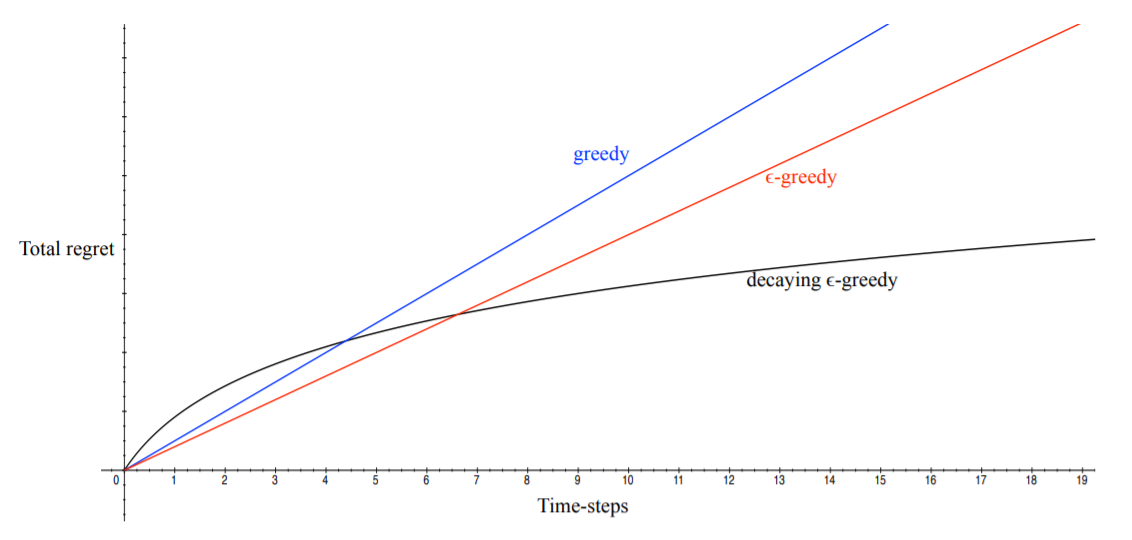
\includegraphics[width=10cm]{regret-over-time}
	\caption{Total regret over time}
	\label{fig:regret-over-time}
\end{figure}

From \ref{fig:regret-over-time}, the following observations can be made. If an algorithm \textit{never}- or \textit{forever} explores, the total regret will be \textit{linear}. This is not good, since the goal is to minimize regret while exploring. The idea of \textit{decaying} $\epsilon$-greedy is interesting, since it will converge to a logarithmic regret.

Lets estimate $Q(a) \approx \hat{Q}_t(a)$. The value of each action can be evaluated by MC-evaluation: $\hat{Q}_t(a) = \frac{1}{N_t(a)} \sum_{t = 1}^{T} r_t 1(a_t = a)$.

Since the \textit{greedy} algorithm always selects the action with the highest value, it can lock onto a sub-optimal action forever, thus receiving a linear total regret.

Using an \textit{$\epsilon$-greedy} algorithm, the constant $\epsilon$ ensures that the minimum regret $l_t \geq \frac{\epsilon}{A} \sum_{a \in A} \Delta_a$. Thus, the total regret is also linear.

A simple but powerful idea is to use \textbf{Optimistic Initialization}. Initialize $Q(a)$ to a very high value and from there on update the action-value by MC evaluation starting with $N(a) > 0$. It encourages exploration early on, but can still lock onto sub-optimal actions. In practice however, this generally works really well.

The \textit{decaying $\epsilon$-greedy} algorithm works by picking a decaying schedule for $\epsilon_1, \epsilon_2, ...$. Imagine the following schedule
\begin{equation*}[
	\begin{aligned}
		c & > 0\\
		d & = \min_{a | \Delta_a > 0} \Delta_i\\
		\epsilon_t & = \min \{1, \frac{c|A|}{d^2t}\}
	\end{aligned}
\end{equation*}

There is a problem with the schedule though. It uses advance knowledge about gaps. So, the goal is to find an algorithm with sub-linear regret for any multi-armed bandit without using knowledge of $R$.

The performance of any algorithm is determined by the \textit{similarity} between the optimal arm and other arms. Hard problem have similar-looking arms with different means. This can be described as the size of the gap, and the similarity in distributions (measure by KL-divergence).

The following \textbf{Lower Bound} is a theorem. It means the \textit{asymptotic total regret is at least logarithmic in the number of steps}.

\begin{equation*}
	\lim_{t \rightarrow \infty} L_t \geq \log t \sum_{a | \Delta_a > 0} \frac{\Delta_a}{KL(R^a||R^{a^*})}
\end{equation*}

\subsection{Upper Confidence Bounds}

\begin{figure}[H]
	\centering
	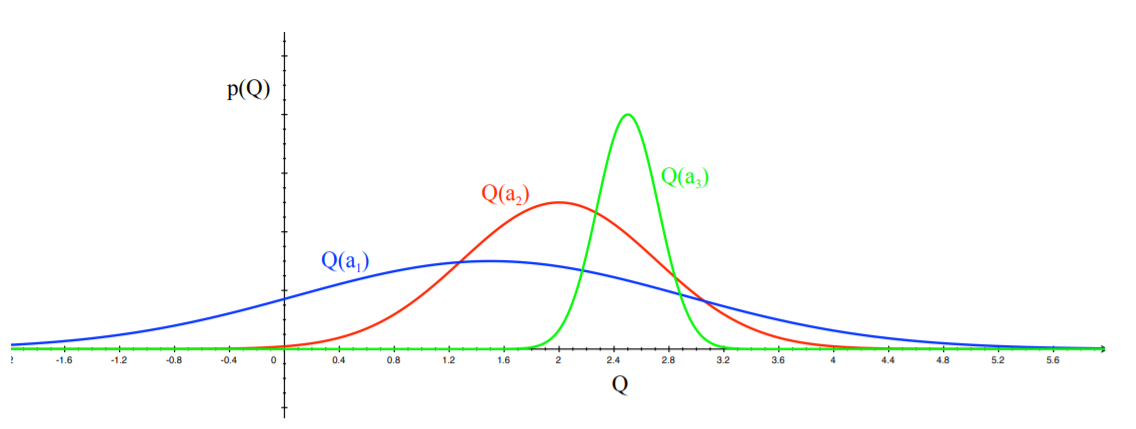
\includegraphics[width=10cm]{oitfou-before}
\end{figure}

Take a look at the figure above. The idea of \textbf{Optimism in the Face of Uncertainty} is to pick the action with the highest potential. This would be $a_1$, since the tail of the distribution is the best one of them all. Say you pick this action. Then, the distribution gets updated.

\begin{figure}[H]
	\centering
	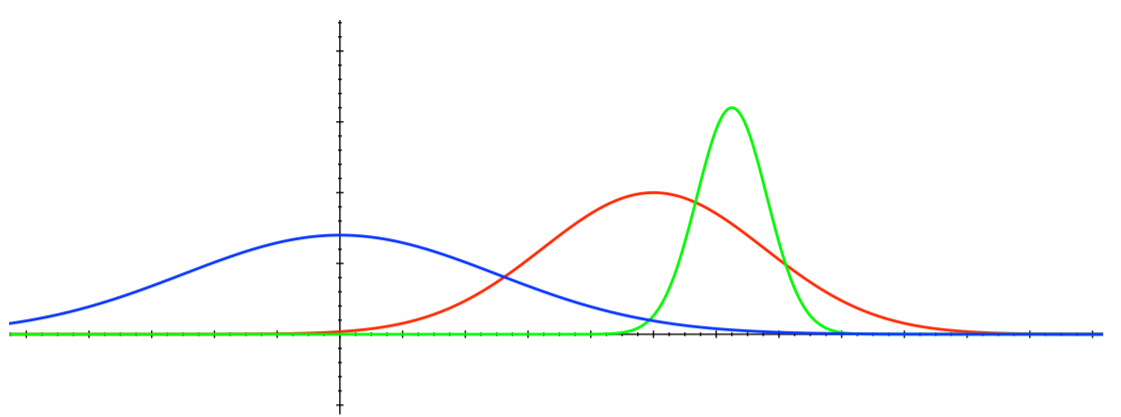
\includegraphics[width=10cm]{oitfou-after}
\end{figure}

Now, we are more certain about the actual value of $Q(a_1)$ and thus more likely to pick another action until the optimal one has been discovered.

Another way to estimate uncertainty is through \textbf{Upper Confidence Bounds} (UCB). An upper confidence $\hat{U}_t(a)$ can be calculated for each action-value, such that $Q(a) \leq \hat{Q}_t(a) + \hat{U}_t(a)$ with high probability. The action maximizing the UCB is then selected.

By \textbf{Hoeffding's Inequality}, $\Prob\left[\E\left[X\right] > \bar{X}_t + u\right] \leq e^{-2tu^2}$ for $\bar{X}_t = \frac{1}{T} \sum_{t = 1}^T X_t$, where $X_t$ is an i.i.d. r.v. in $[0, 1]$. When applying this to the bandit problem, the following can be derived

\begin{equation*}
	\Prob\left[Q(a) > \hat{Q}_t(a) + U_t(a)\right] \leq e^{-2N_t(a)U_t(a)^2}
\end{equation*}

Now, pick a probability $p$ that the true value exceeds the UCB.

\begin{equation*}
	\begin{aligned}
		p & = e^{-2N_t(a)U_t(a)^2}\\
		U_t(a) & = \sqrt{\frac{-\log p}{2 N_t(a)}}
	\end{aligned}
\end{equation*}

Since the goal is to reduce the probability as more rewards are observed, set e.g. $p = t^{-4}$. Then ensures the optimal action is selected when $t \rightarrow \infty$. The final equation becomes

\begin{equation*}
	U_t(a) = \sqrt{\frac{2 \log t}{N_t(a)}}
\end{equation*}

This leads to the \textbf{UCB1} algorithm

\begin{equation*}
	a_t = \arg\max_{a \in A} Q(a) + \sqrt{\frac{2 \log t}{N_t(a)}}
\end{equation*}

\textit{Theorem}: the UCB algorithm achieves logarithmic asymptotic total regret
\begin{equation*}
	\lim_{t \rightarrow \infty} L_t \leq 8 \log t \sum_{a | \Delta_a > 0} \Delta_a
\end{equation*}

\subsection{Bayesian Bandits}

So far, no assumptions were made about the reward distribution $R$, except for bounds on rewards. \textbf{Bayesian Bandits} exploit prior knowledge of rewards, $p\left[R\right]$. They compute the posterior distribution of reward $p\left[R | h_t\right]$, where $h_t = a_1, r_1, ..., a_{t-1}, r_{t-1}$ is the history. The posterior distribution can then be used to guide exploration.

The following is an example. Assume that the reward distribution is Gaussian, so $R_a(r) = N(r; \mu_a, \sigma_a^2)$. The Gaussian posterior over $\mu_a$ and $\sigma_a^2$ can be computed using Bayes' law: $p[\mu_a, \sigma_a^2; h_t] \propto p[\mu_a, \sigma_a^2] \prod_{t | a_t = a} N(r_t; \mu_a, \sigma_a^2)$.

Then, pick the action that maximizes the standard deviation of $Q(a)$, so $a_t = \arg\max_{a \in A} \mu_a + \frac{c \sigma_a}{\sqrt{N(a)}}$. This is a Bayesian way to compute Upper Confidence Bounds.

\begin{figure}[H]
	\centering
	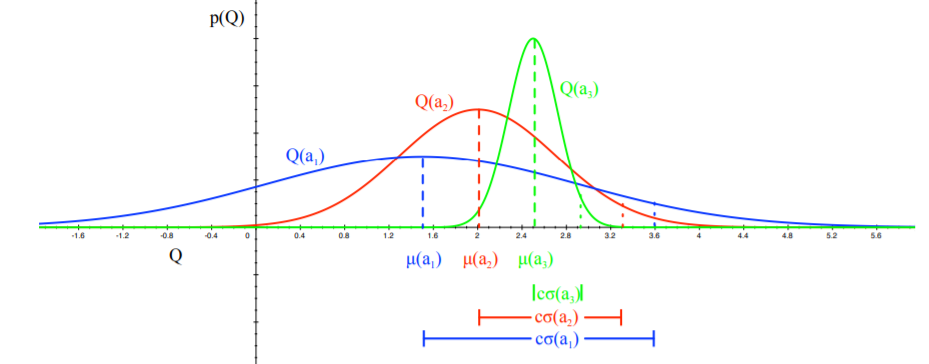
\includegraphics[width=10cm]{ucb-bayesian}
\end{figure}

Here, the blue action would be taken. This is because the mean and standard deviation summed up is the largest (assuming an equal number of visits).

\subsection{Probability Matching}

\textbf{Probability Matching} selects an action $a$ according to the probability that $a$ is optimal. It can be calculated using
\begin{equation*}
	\pi(a) = \Prob \left[Q(a) = \max_{a'} Q(a') | R_1, ..., R_{t-1}\right]
\end{equation*}
This concept is optimistic in the face of uncertainty, since uncertain actions have a higher probability of being the maximum. A disadvantage however is that it can be difficult to be computed analytically from the posterior.

\textbf{Thompson Sampling} is sample-based probability matching. The policy can be computed using
\begin{equation*}
	\pi(a) = \E\left[1(Q(a) = \max_{a'} Q(a')) | R_1, ..., R_{t-1}\right]
\end{equation*} 
Then, use Bayes' law to compute the posterior distribution $P_w(Q|R_1, ..., R_{t-1})$. First sample an action-value $Q(a)$ from the posterior. Then, choose action $A_t = \arg\max_{a \in A} Q(a)$.

\subsection{Information State Search}

The goal of exploration is to gain more information about the environment. If it is possible to quantify how much this information is worth. When this value is known, the optimal trade-off between exploration and exploitation is known.

The idea is to look at bandits as \textit{sequential} decision-making processes instead of \textit{one-step}. At each step, there is an \textbf{information state} $\bar{s} = f(h_t)$. So, the state is a summary of all history that has been accumulated so far. Each action $a$ then causes a transition to a new information state $\bar{s}'$, with probability $\bar{P}^a_{\bar{s}\bar{s}'}$.

This defines the MDP $\bar{M}$ in augmented information state space $\bar{M} = (\bar{S}, A, \bar{P}, R, \gamma)$.

An example of this are Bernoulli Bandits, so lets say $R^a = Bernoulli(\mu_a)$. The goal is to find the arm with the highest $\mu_a$. The information state space $\bar{s} = (\alpha, \beta)$, where $\alpha_a$ and $\beta_b$ count when the reward was 0 or 1 respectively.	 This MDP can then be solved by previously discussed Reinforcement Learning algorithms. There is an alternative approach, referred to as \textbf{Bayes-adaptive RL}. For Bernoulli bandits, it finds the Bayes-optimal exploration/exploitation trade-off with respect to the prior distribution.

Imagine a problem of drug assignment. There are two drugs 1 and 2 that can be used; $\bar{s} = (\alpha_1, \beta_1, \alpha_2, \beta_2)$. First, start with a $Beta(\alpha_a, \beta_a)$ prior over reward function $R^a$. Each time $a$ is selected, the distribution gets updated accordingly, since a success will increase beta, and a failure increases alpha. Here, each state transition corresponds to a Bayesian model update. 

The solution of this problem is known as the \textit{Gittens} index, and can be computed by solving the MDP (by using for example MCTS for planning).

\section{Contextual Bandits}

A \textbf{Contextual Bandit} is a tuple $(A, S, R)$. Instead of the bandit problem, there is now also a state space, which provides \textit{context} to the problem. $S = \Prob[s]$ is an unknown distribution over the contexts. Then, the reward $R^a_s(r) = \Prob[r|s, a]$ is an unknown probability distribution of the rewards. At each time step, the environment generates $s_t \sim S$. Then, an agent selects $a_t \in A$, to which the environment generates $r_t \sim R^{a_t}_{s_t}$. The goal is to maximize $\sum_{T=1}^t r_T$.

This section explains the concept of \textbf{Linear UCB}. The action-value function needs to be estimated: $Q(s, a) = \E[r|s,a] \approx Q_\theta(s, a) = x(s, a)^\intercal \theta$. The parameters of this linear function can be estimated by least-squares. The solution is
\begin{equation*}
	\theta_t = \left(\sum_{T=1}^t x(s_T, a_T)x(s_T, a_T)^\intercal\right)^{-1} \sum_{T=1}^t x(s_T, a_T)r_T
\end{equation*}

Least squares regression estimates $Q_\theta(s, a)$. However, it can also be used to estimate the variance of the action-value $\sigma^2_\theta(s, a)$. The idea is to add a bonus for uncertainty, $U_\theta(s, a) = c\sigma$, where the UCB is the number of standard deviations above the mean defined by $c$.

For least squares regression, parameter covariance is $A^{-1} = \left(\sum_{T=1}^t x(s_T, a_T)x(s_T, a_T)^\intercal\right)^{-1}$. The action-value is linear in features, so

\begin{equation*}
	\begin{aligned}
		\sigma^2_\theta(s, a) & = x(s, a)^\intercal A^{-1} x(s, a)\\
		a_t & = \arg\max_{a \in A} Q_\theta(s_t, a) + c\sigma_\theta(s_t, a)\\
		a_t & = \arg\max_{a \in A} Q_\theta(s_t, a) + c \sqrt{x(s, a)^\intercal A^{-1} x(s, a)}
	\end{aligned}
\end{equation*}

\section{MDPs}

All previously described principles for exploration/exploitation can apply to MDPs with slights modifications.

\begin{itemize}
	\item Optimistic Initialization
	\begin{itemize}
		\item Model-Free RL
		
		The idea is to initialize $Q(s, a)$ to $\frac{r_{max}}{1 - \gamma}$. This encourages systematic exploration of states and actions.
		\item Model-Based RL
		
		Here, an optimistic model of the MDP is constructed. For example, transitions to a terminal state are initialized with $r_{max}$ reward. An example is the RMax algorithm (Brafman and Tennenholtz).
	\end{itemize}

	\item Optimism in the Face of Uncertainty
		\begin{itemize}
		\item Model-Free RL
		
		The goal is to maximize UCB on the action-value function $Q^\pi(s, a)$. $a_t = \arg\max_{a \in A} Q(s_t, a) + U(s_t, a)$. It estimates uncertainty in policy evaluation. However, it completely ignores uncertainty in the policy improvement step.
		
		For this reason, maximize UCB on $Q^*(s, a)$ instead. $a_t = \arg\max_{a \in A} Q(s_t, a) + U_1(s_t, a) + U_2(s_t, a)$. This estimates uncertainty in both policy evaluation and policy improvement. However, estimating policy improvement uncertainty is hard to do.		
		
 		\item Model-Based RL
		
		Bayesian Model-Based RL maintains a posterior distribution over MDP models. Both transitions and rewards are estimated $p[P, R| h_t], h_t = s_1, a_1, r_2, ..., s_t$. This posterior can then be used to guide exploration by for example Bayesian UCB or Thompson Sampling.
	\end{itemize}

	\item Probability Matching
	
	Thompson sampling implements probability matching
	\begin{equation*}
		\begin{aligned}
			\pi(s, a | h_t) & = \Prob[Q^*(s, a) > Q^*(s, a'), \forall a' \neq a | h_t]\\
							& = \E_{P, R| h_t}\left[1(a = \arg\max_{a \in A} Q^*(s, a))\right]
		\end{aligned}
	\end{equation*}

	Bayes' Law can be used to compute posterior distribution $p[P, R| h_t]$. Then, sample an MDP $P, R$ from the posterior. Then, solve this MDP using a favored planning algorithm to obtain $Q^*(s, a)$. Then, select the optimal action from the sample MDP by $a_t \arg\max_{a \in A} Q^*(s_t, a)$. 
		
	\item Information State Search
	
	MDPs can also be augmented to include an information state. The augmented state becomes $(s, \hat{s})$, where $s$ is the original state within the MDP, and $\hat{s}$ is accumulated information about the history. Each action $a$ causes a transition to $s'$ with probability $P^a_{ss'}$. However, a new information state $\hat{s}'$ is also created.
	
	The posterior distribution over the MDP model is an information state $\hat{s_t} = \Prob[P, R| h_t]$. An augmented MDP over $(s, \hat{s})$ is called a \textbf{Bayes-Adaptive MDP}.
	
	Solving this MDP gives rise to the optimal exploration/exploitation trade-off. However, the Bayes-Adaptive MDP is typically enormous. Simulation-based search has been proven effective to this problem.
\end{itemize}